\documentclass[12pt, letterpaper]{../assignment}
\usepackage{graphicx}
\usepackage{courier}
\usepackage{minted}
\usepackage{amsmath}
\usepackage{commath}
\usepackage{amssymb}
\usepackage{amsfonts} 
\usepackage{cancel}


\usemintedstyle{monokai}
\oddsidemargin = 0pt
\exercisesheet{Module 2}{Practice Assignment}
\student{Austin Barrilleaux}
\courselabel{EN 525.609}
\semester{Fall 2023}
\usepackage[backend=bibtex,style=numeric,sorting=none]{biblatex}
\bibliography{reference}
\usepackage{color}
\definecolor{light-gray}{rgb}{0.2,0.2,0.2}
\setminted{bgcolor=light-gray}
\setlength{\parindent}{0pt}

\makeatletter
\patchcmd{\minted@colorbg}{\noindent}{\medskip\noindent}{}{}
\apptocmd{\endminted@colorbg}{\par\medskip}{}{}
\makeatother

\begin{document}
\subsection*{Problem 1}
\subsubsection*{Solve the following practice problems in the 9th edition textbook.\\
\begin{itemize}
    \item Chapter 3:
    \begin{itemize}
        \item 3-12(a)
    \end{itemize}
\end{itemize}}

\subsubsection*{The block diagram of an electric train control is shown in  Fig. \ref{Fig:prob3_12}. The system parameters and variables are:
\begin{itemize}
    \item $e_r(t) = $ voltage representing the desired train speed, $V$
    \item $v(t) = $ speed of train, ft/sec
    \item $M = $ Mass of train $=$ 30,000 lb/sec$^2$
    \item $K = $ amplifier gain
    \item $k_t = $ gain of speed indicator = 0.15 V/ft/sec  
\end{itemize}}

\begin{figure}[H]
    \centering
    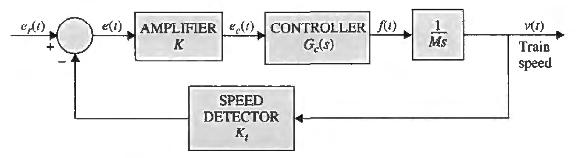
\includegraphics[scale=0.5]{figures/fig_3_12.png}
    \caption{Problem 3-12}
    \label{Fig:prob3_12}
\end{figure}

\subsubsection*{To determine the transfer function of the controller, we apply a step function of 1 volt to the input of the controller, that is, $e_c(t) = u_s(t)$.
The output of the controller is measured and described by the following equation:}

$$ f(t) = 100(1 - 0.3 e^{-6t} - 0.7 e ^{-10t}) u_s (t) $$

\subsubsection*{(a) Find the transfer function $G_c(s)$ of the controller.}

From Fig. \ref{Fig:prob3_12}, we can see that:

$$ \frac{F(s)}{E_c(s)} = G_c(s) $$

Since:

$$ f(t) = 100(1 - 0.3 e^{-6t} - 0.7 e ^{-10t}) u_s (t) $$

Then using the Laplace Transform Table from the book:

$$ F(t) = \mathcal{L}^{-1} \left[100 - 30 e^{-6t} - 70 e ^{-10t}\right]  =
\frac{100}{s} - \frac{30}{s+6} - \frac{70}{s+10} $$

To get a common denominator for $F(t)$:

$$ F(t) =
\frac{100(s+6)(s+10) - 30s(s+10)  - 70s(s+6)}{s(s+6)(s+10)} $$

$$ F(t) =
\frac{100(s^2+16s+60) - 30(s^2+10s)  - 70(s^2+6s)}{s(s+6)(s+10)} $$

$$ F(t) =
\frac{100(16s+60) - 30(10s)  - 70(6s)}{s(s+6)(s+10)} $$

$$ F(t) =
\frac{880s + 6000}{s(s+6)(s+10)} $$

$$ F(t) =
\frac{880\left(s + \frac{600}{88}\right)}{s(s+6)(s+10)} $$

Since:

$$ e_c(t) = u_s (t) $$

Then using the Laplace Transform Table from the book:

$$ E_c(s) = \mathcal{L}^{-1} \left[u_s (t)\right]  =
\frac{1}{s} $$

Using these, $G_c(s)$ is:

$$ G_c(s) = \frac{F(s)}{E_c(s)} =
\frac{\frac{880\left(s + \frac{600}{88}\right)}{s(s+6)(s+10)}}{\frac{1}{s}} $$

Or more simply:

\begin{answer}
    $$ G_c(s) = 
    \frac{880\left(s + \frac{600}{88}\right)}{(s+6)(s+10)} $$
\end{answer}

\subsubsection*{(b) Derive the forward-path transfer function $\frac{V(s)}{E(s)}$ of the system.
The feedback path is opened in this case.}

From Fig. \ref{Fig:prob3_12}, we can see that:

$$ \frac{V(s)}{E(s)} = K G_c(s) \frac{1}{M s} $$

Given the values for $G_c(s)$ and $M$ from part (a) and the problem prompt respectively,
and the fact that there is no value for $K$:

$$ \frac{V(s)}{E(s)} = K \frac{880\left(s + \frac{600}{88}\right)}{(s+6)(s+10)} \frac{1}{30,000 s} $$

$\frac{V(s)}{E(s)}$ can be written as:

\begin{answer}
$$ \frac{V(s)}{E(s)} = \frac{880 K \left(s + \frac{600}{88}\right)}{30,000 s(s+6)(s+10)} $$
\end{answer}

\subsubsection*{(c) Derive the closed-loop transfer function $\frac{V(s)}{E_r(s)}$ of the system.}

Using block diagram reduction techniques, we can get that the transfer function is:

$$ \frac{V(s)}{E_r(s)} =  \frac{K G_c(s) \frac{1}{M s}}{1 + K G_c(s) \frac{1}{M s}K_t} $$

Which can be more simply written as:

$$ \frac{V(s)}{E_r(s)} =  \frac{K G_c(s)}{M s + K G_c(s) K_t} $$

Given the values for $G_c(s)$ from part (a) and $M$ and $K_t$ from the problem prompt,
and the fact that there is no value for $K$:

$$ \frac{V(s)}{E_r(s)} = 
\frac{K \frac{880\left(s + \frac{600}{88}\right)}{(s+6)(s+10)}}{30,000 s + K \frac{880\left(s + \frac{600}{88}\right)}{(s+6)(s+10)} 0.15} $$

Which can be simplified to:

$$ \frac{V(s)}{E_r(s)} = 
\frac{K 880\left(s + \frac{600}{88}\right)}{30,000 s(s+6)(s+10) + K 880\left(s + \frac{600}{88}\right) 0.15} $$

Further:

$$ \frac{V(s)}{E_r(s)} = 
\frac{K \frac{88}{3000}\left(s + \frac{600}{88}\right)}{s(s+6)(s+10) + K \frac{88}{3000}\left(s + \frac{600}{88}\right) 0.15} $$

Expanding the denominator, the closed-loop transfer function $\frac{V(s)}{E_r(s)}$ of the system is:

\begin{answer}
$$ \frac{V(s)}{E_r(s)} = 
\frac{K \frac{88}{3000}\left(s + \frac{600}{88}\right)}{s^3+16s^2 + s \left(K\frac{44}{10000}+ 60\right) + K \frac{3}{100} } $$
\end{answer}

\subsubsection*{(c) Assuming that K is set at a value so that the train will not run away (unstable),
find the steady-state speed of the train in feet per second when the input is $e_r(t) = u_s(t) V$.}

The speed of train, $v(t)$ will approach a value at steady state when $t \rightarrow \infty$.
Therefore we must solve the limit:

$$ \lim_{t\to+\infty} v(t) = v_{ss} $$

Given $e_r(t) = u_s(t) V$:

$$E_r(s) = \frac{1}{s}$$

If we substitute this into the transfer function from part (c), we get the following:

$$ s V(s) = 
\frac{K \frac{88}{3000}\left(s + \frac{600}{88}\right)}{s^3+16s^2 + s \left(K\frac{44}{10000}+ 60\right) + K \frac{3}{100} } $$

From the final value theorem we know that:

$$ \lim_{t\to+\infty} f(t) = \lim_{s\to 0} s F(s) $$

Therefore:

$$ \lim_{t\to+\infty} v(t) = \lim_{s\to 0} s V(s) = v_{ss} $$

So:

$$ v_{ss} = \lim_{s\to 0} \frac{K \frac{88}{3000}\left(s + \frac{600}{88}\right)}{s^3+16s^2 + s \left(K\frac{44}{10000}+ 60\right) + K \frac{3}{100} } $$

Analyzing the limit:

$$ v_{ss} = \frac{K \frac{88}{3000}\left(\frac{600}{88}\right)}{K \frac{3}{100} } =
\frac{\frac{600}{3000}}{\frac{3}{100} } = \frac{20}{3}  $$

The steady-state speed of the train is:

\begin{answer}
$$ v_{ss}(t) = \frac{20}{3} \text{ft/s}  $$
\end{answer}

\subsection*{Problem 2}

\subsubsection*{Using Mason's Gain Formula,
determine the transfer function from input $R(s)$ to output $Y(s)$ given the following signal flow graph:}

\begin{figure}[H]
    \centering
    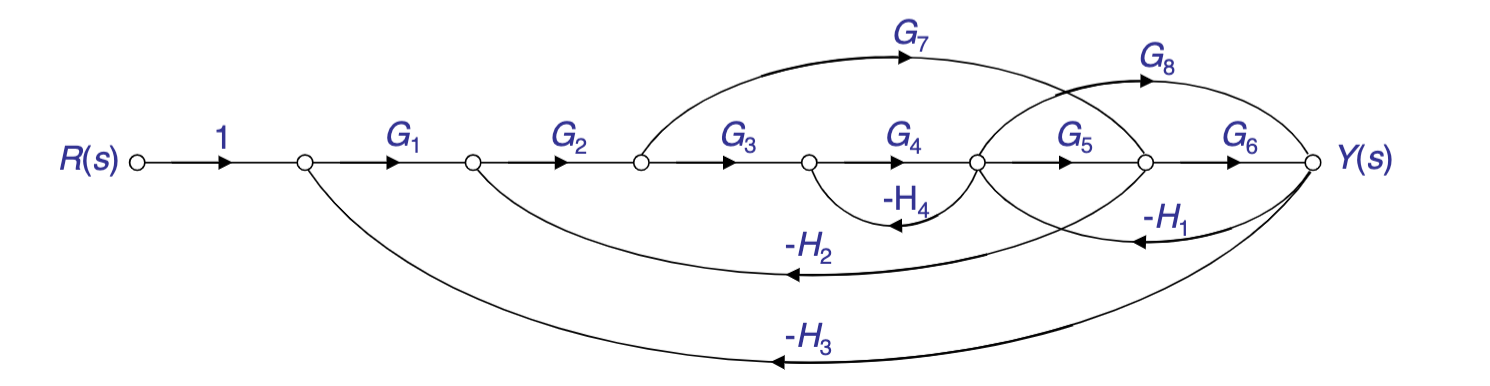
\includegraphics[scale=0.5]{figures/Problem_2_sfd.png}
    \caption{Problem 2: Signal Flow Graph}
    \label{Fig:sfg}
\end{figure}

There are three forward paths:

$$ M_1 = G_1 G_2 G_3 G_4 G_5 G_6 $$

$$ M_2 = G_1 G_2 G_7 G_6 $$

$$ M_3 = G_1 G_2 G_3 G_4 G_8 $$

There are four loops:

$$ L_{11} = G_5 G_6 (-H_1) $$

$$ L_{21} = G_2 G_3 G_4 G_5 (-H_2) $$

$$ L_{21} = G_1 G_2 G_3 G_4 G_5 G_6 (-H_3) $$

$$ L_{41} = G_4 (-H_4) $$

All loops touch $M_1$ and $M_3$:

$$ \Delta_1 = \Delta_3  = 1 $$

Loop $M_2$ does not touch $L_{41}$:

$$ \Delta_2 = 1 - L_{41} $$

Pairs of non-touching loops are:

\begin{itemize}
    \item $L_{11}$ does not touch $L_{21}$
    \item $L_{21}$ does not touch $L_{31}$
    \item $L_{21}$ does not touch $L_{41}$
    \item $L_{31}$ does not touch $L_{41}$
\end{itemize}

Triplets of non-touching loops are:

\begin{itemize}
    \item $L_{21}$, $L_{31}$ and $L_{41}$ share no common nodes
\end{itemize}

$\Delta$ is calculated as:
$$ \Delta = 1 - (L_{11}+L_{21}+L_{31}+L_{41}) + (L_{11}L_{21} + L_{21}L_{31} + L_{21}L_{41} + L_{31}L_{41} ) - (L_{21} L_{31} L_{41})$$

Therefore, the Transfer Function is:
{\footnotesize
\begin{answer}
$$ M = \frac{Y(s)}{R(s)} = \frac{M_1 + M_2 (1 - L_{41}) + M_3}{1 - (L_{11}+L_{21}+L_{31}+L_{41}) + (L_{11}L_{21} + L_{21}L_{31} + L_{21}L_{41} + L_{31}L_{41} ) - (L_{21} L_{31} L_{41})} $$
\end{answer}
}

\subsection*{Problem 3}
\subsubsection*{Consider the multivariable feedback system below and compute the multivariable closed-loop transfer function}

\begin{figure}[H]
    \centering
    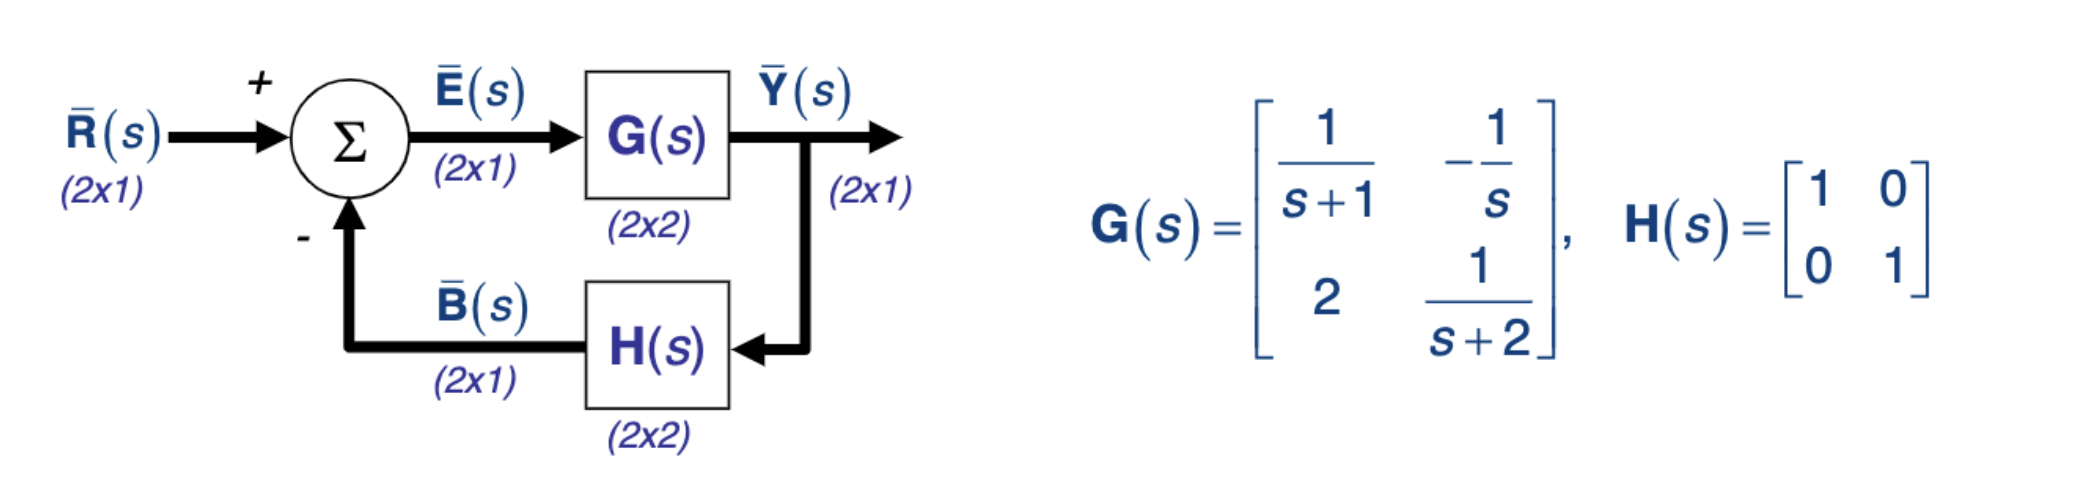
\includegraphics[scale=0.4]{figures/mutivar_feedback_system.png}
    \caption{Problem 3: Multivariable Feedback System}
    \label{Fig:mvfs}
\end{figure}

The transfer function of the closed loop transfer function is:

$$\frac{Y(s)}{R(s)} = \frac{G(s)}{1+G(s)H{s}} $$

$G(s)H{s}$ is calculated as:

$$G(s)H{s} = G(s) = \left(\begin{array}{cc} \frac{1}{s+1} & -\frac{1}{s}\\ 2 & \frac{1}{s+2} \end{array}\right)$$

Therefore:

$$ 1 + G(s)H{s} = 1 + G(s) = \left(\begin{array}{cc} 1 + \frac{1}{s+1} & 1-\frac{1}{s}\\ 3 & 1 + \frac{1}{s+2} \end{array}\right) $$

Getting common denominators:

$$ 1 + G(s)H{s} = \left(\begin{array}{cc} \frac{s+2}{s+1} & \frac{s-1}{s}\\ 3 & \frac{s+3}{s+2} \end{array}\right) $$

The inverse of which is:

$$ [1 + G(s)H{s}]^{-1} = \frac{1}{(\frac{s+2}{s+1})(\frac{s+3}{s+2}) - 3\frac{s-1}{s} } \left(\begin{array}{cc} \frac{s+3}{s+2} & -\frac{s-1}{s}\\ -3 & \frac{s+2}{s+1}  \end{array}\right)
= \frac{s(s+1)}{s(s+3)-3(s+1)(s-1)}  \left(\begin{array}{cc} \frac{s+3}{s+2} & -\frac{s-1}{s}\\ -3 & \frac{s+2}{s+1}  \end{array}\right) $$

Which becomes:

$$ [1 + G(s)H{s}]^{-1} 
= \frac{s(s+1)}{- 2 s^2 + 3 s + 3}  \left(\begin{array}{cc} \frac{s+3}{s+2} & -\frac{s-1}{s}\\ -3 & \frac{s+2}{s+1}  \end{array}\right) $$

Therefore, the transfer function is:

$$ \frac{Y(s)}{R(s)}
= \frac{s(s+1)}{- 2 s^2 + 3 s + 3} \left(\begin{array}{cc} \frac{1}{s+1} & -\frac{1}{s}\\ 2 & \frac{1}{s+2} \end{array}\right)  \left(\begin{array}{cc} \frac{s+3}{s+2} & -\frac{s-1}{s}\\ -3 & \frac{s+2}{s+1}  \end{array}\right) $$

Or:

$$ \frac{Y(s)}{R(s)}
= \frac{s(s+1)}{- 2 s^2 + 3 s + 3} \left(\begin{array}{cc} \frac{1}{s+1}\frac{s+3}{s+2} +3\frac{1}{s} & -\frac{1}{s+1}\frac{s-1}{s} -\frac{1}{s}\frac{s+2}{s+1}\\ 2\frac{s+3}{s+2} -3\frac{1}{s+2} & -2\frac{s-1}{s} + \frac{1}{s+2}\frac{s+2}{s+1} \end{array}\right)  $$

Simplifying:

$$ \frac{Y(s)}{R(s)}
= \frac{s(s+1)}{- 2 s^2 + 3 s + 3} \left(\begin{array}{cc} \frac{s(s+3)+3(s+1)(s+2)}{s(s+1)(s+2)}  & -\frac{2s+1}{s(s+1)} \\ \frac{2s+3}{s+2} & \frac{s(s+2)-(2s-2)(s+1)(s+2)}{s(s+1)(s+2)}  \end{array}\right)  $$

Simplifying one last time, we get that the closed loop transfer function is:

\begin{answer}
$$ \frac{Y(s)}{R(s)}
= \frac{1}{- 2 s^2 + 3 s + 3} \left(\begin{array}{cc} \frac{2(2 s^2 + 6s + 3)}{(s+2)}  & -2s+1 \\ \frac{(2s^2+3s)(s+1)}{s+2} & - 2 s^2 + s + 2  \end{array}\right)  $$
\end{answer}

\end{document}

